
\indent\textbf{\emph{Paradigm shift in computing.}}
Growing demand to perform large-scale computations influences changes in organizaton of underlying computational infrastructure.
Hardware-related implementation details of data centers has been the subject to refinement from the earliest days of computing.
Concurrently, the software that manages the operation of data center evolved, further influencing the way data centers are structured and the way clients interact with them.
Improvements in task isolation, resource sharing and transparent concurrency encouraged growth of data centers' processing capabilities.
The software advancements played the primal role in allowing the increase in computational power of data centers without wasting its resources.
Computational tasks require multiple types of resources to complete: CPU time, memory, I/O operations and network bandwith.
Needs for resources often vary in time and are unpredictable or expensive to predict.
Co-existence of multiple tasks in the data center allows to compensate for the variable demand for resources in computational tasks by resource-aware scheduling.
Such techniques are especially useful (but not limited to) in computationally-intensive applications, where the response time is not the primary concern.
Examples of such applications include
engineering (material modelling, electronic circuits optimization),
computational biology and chemistry (protein folding, DNA sequence matching),
physics (fluid dynamics, seach for exoplanets, weather and climate prediction),
and wide range of optimization for military and industry (packing and covering, data mining, economics, artificial intelligence).

\textbf{\emph{Outsourcing computations.}}
Growth of data center influences not only the physical implementation of its infrastructure, but also its ownership by specialied companies, geographical location \& outside-world connectivity and the way clients interact with them.
Modern general-purpose and open for general use data centers such as Microsoft Azure \cite{url-azure}, Amazon Elastic Cloud Computing EC2 \cite{url-amazon-ec2} or Google Compute Engine \cite{url-gce} provide on-demand computational power while hiding most of details concerning resource management.

From the perspective of the client, outsourcing computations provides a wide range of benefits.
It is possible to avoids costs of infrastructure management and maintenance, which is crucial for computational tasks that arise occasionally.
If the demand for resources increases unexpectedly, it can be immediately provided without physical extension of the infrastructure.
Existance of competition in data center market provides security and competitive pricing.

From the perspective of the infrastructure owner, multitude of problems and requirements arise: security in resource-sharing scenerios, standarization and compatibility, automation, availability, extensibility and modularity, recovery, and many more.
An important class of new challenges in data center is optimization of running costs.
Processing speed can scale down to save energy, read-only memory can be shared or distributed, and cooperating processes can migrate closer in the network to save bandwidth.


\textbf{\emph{Modern technologies in data center management.}}

A particular piece of technology that suits the model of modern data center extraordinarly well is virtualization.
Virtualization provides an abstraction layer, called the \emph{virtual machine} for the underlying hardware of a computer system.
Such virtual machine mimics functionality of the physical hardware so closely and directly that it can be used as an environment for a complete operating system.
Such operating system, running on a virtual machine is called the \emph{guest operating system}, which operates in additon to the \emph{host operating system}, which operates on the physical hardware.

(virtualization suits clients)
Guest operating system's perspective is restricted to such exposed virtual machine and is provided with an illusion of possesing the whole computer system.
One of main features of virtualization in datacenter is to provide the complete and non-restricted environment for the client that is isolated from the management software and other clients' tasks.

(virtualization suits data center owners)
Besides providing an abstraction layer, virtualization provides several control features.
Absolute control over the underlying, virtual hardware of the guest operating system allows to suspend and resume the execution of the guest operating system.
Such functionality provides building blocks for the feature of migration, which transfers the complete virtual machine to a different physical machine.
Possibility of migration plays an important role in load balancing in the data center and allows for sophisticated optimizations such as reducing network distance between communicating virtual machines.

Data center consists of multiple virtual machines running on physical nodes that are connected by physical network.
Data centers provide its resources to the clients as the set of virtual machines connected by a virtual network.
Cooperation over the network. Network reservations.

Virtualization allows to be flexible in renting infrastructure. But poses new challenges in datacenters.
Existing virtualization solutions: XEN.

\textbf{\emph{New challenges.}}

Problem central to this thesis

\begin{center}
  \emph{How to assign virtual machines to physical machines in the datacenter?}
\end{center}

We elaborate more in subsequent subsection.

\section{Not covered}


\begin{itemize}
  \item
Variety of types of computations are endless, but certain applications are known to consume as much computational power as it is provided: protein folding, weather prediction, economic systems analysis, artificial intelligence and data mining, material modelling, drug design, DNA sequence matching, drug design, search for Exo-planets, fluid dynamics, military, optimization for industries etc.
\item The topology of multiple computers: set of computers connected by the network.
\item Parallelism as a consequence of Moore's law diminish for single core (physical limitations on size of electronic circuts).
\end{itemize}


\section{SEPARATOR}

\section{Algorithmic challenges of the virtual machines embedding}

In this thesis we consider two scenarios:
\begin{enumerate}
  \item the communication pattern among virtual machines is known up-front
  \item the communication pattern is not known, and has to be discovered and is a subject to changes over time
\end{enumerate}

\section{Network optimization}

TODO Tree Caching

\section{Performance metrics}

Methods of Measuring the Quality of Results

\subsection{Online Algorithms and Competitive Analysis}

Sleator, Tarjan: list update \cite{competitive-analysis}
Borodin book \cite{borodin-book}

\subsection{Time and Space Complexity and NP-completeness}


\section{Bibliographic notes}

\section{Outline of the Thesis}

Organization of the ``paper'', how connected the chapters are.

\section{Contribution of This Thesis}

\subsection{Contributions on static mapping}

This paper initiates the formal study of data-locality and replica aware virtual network embedding problems in datacenters.
In particular, we decompose the general optimization problem into its fundamental aspects, such as
assignment of chunks, replica selection, and flexible virtual machine
placement, and answer questions such as:
\begin{enumerate}
\item Which chunks to assign to which virtual machine?

\item How to exploit redundancy and select good replicas?

\item How to efficiently embed virtual machines and their inter-connecting network?

\item Can the chunk assignment, replica selection and virtual machine embedding problems be jointly optimized, in polynomial time?
\end{enumerate}

We draw a complete picture of the problem space: We show that
even problem variants exhibiting multiple degrees of freedom in terms of
replica selection and embedding,
can be solved optimally in polynomial time, and we present several efficient
algorithms accordingly. However, we also prove limitations in terms of
computational tractability, by providing reductions from 3-D matching
and Boolean satisfiability ($\SAT$). Interestingly,
while it is well-known that (unsplittable) multi-commodity flow
problems are NP-hard in capacitated networks, our hardness results also hold in \emph{uncapacitated}
networks; moreover, we show that NP-hard problems already arise in small-diameter networks (as they are
widely used today~\cite{fattree}).

\subsection{Contribution on dynamic mapping}


This paper introduces the online Balanced RePartitioning problem (BRP),
a fundamental \emph{dynamic} variant of the classic graph clustering problem. 
We show that BRP features some interesting connections to other well-known
online graph problems. For $\ell=2$, BRP is able to simulate online paging problem
and for for $k=2$, BRP is a~novel online version of maximum matching.
We consider deterministic algorithms and make the following technical
contributions:

\begin{description}

\item[Algorithms for General Variant:]
For the non-augmented variant, in \ref{sec:upper}, we first present a~simple
$O(k^2 \cdot \ell^2)$-competitive algorithm. Our main technical contribution
is an $O((1+1/\eps) \cdot k \log{k})$-competitive deterministic algorithm
$\CREP$ for a setting with $(2+\eps)$-augmentation (\ref{sec:crep}).
We emphasize that this bound does not depend on~$\ell$. This is interesting,
as in many application domains of this problem, $k$ is small: for example, in
our motivating virtual machine collocation problem, a server typically hosts
only a small number of virtual machines (e.g., related to the constant number
of cores on the server).

\item[Algorithms for Online Rematching:]
For the special case of online rematching ($k=2$, but arbitrary~$\ell$), in
\ref{sec:k-two}, we prove that a variant of a greedy algorithm is
7-competitive. We also demonstrate a lower bound of 3 for any deterministic
algorithm.

\item[Lower Bounds:]
By a reduction to online paging, in \ref{sec:paging}, we show that
for two clusters no deterministic algorithm can obtain a better bound than
$k-1$. While this shows an~interesting link between BRP and paging, in
\ref{sec:lower-bounds}, we present a stronger bound. Namely, we
show that for $\ell \geq 2$ clusters, no deterministic algorithm can beat the
bound of $k$ even with an~arbitrary amount of augmentation, as~long~as~the
algorithm cannot keep all nodes in a~single cluster. In contrast, online
paging is known to~become constant-competitive with constant
augmentation~\cite{SleTar85}.

\end{description}




\subsection{Contributions on memory management in network devices}

\todo{Mixed with organization of the paper}

We initiate the study of a natural new caching with bypassing problem which
allows to account for tree-dependencies among items. The problem finds
immediate applications, e.g., in IP routing and software-defined networking
(see \lref[Section]{sec:motivation}).

In particular, we consider the online tree caching problem within the resource
augmentation paradigm: we assume that cache sizes of the online algorithm
($\kALG$)  and the optimal offline algorithm ($\kOPT$) may differ. We assume
$\kALG \geq \kOPT$ and let $R = \kALG/(\kALG-\kOPT+1)$.

In \lref[Section]{sec:algo}, we present an elegant deterministic online
algorithm~\ALG for this problem. While our algorithm is simple, its analysis
presented in \lref[Section]{sec:analysis} requires several non-trivial
insights into the problem. In particular, we rigorously prove that \ALG is
$O(h(T) \cdot R)$-competitive, where $h(T)$ is the height of tree~$T$. That
is, we show that there exists a constant~$\beta$, such that $\ALG(I) \leq
O(h(T) \cdot R) \cdot \OPT(I) + \beta$ for any input $I$. Note that this
result is optimal up to the factor~$O(h(T))$: in
\lref[Appendix]{sec:lower-bound-on-the-problem}, we show that the lower
bound~$R$ for the paging problem~\cite{competitive-analysis} implies an
$\Omega(R)$ lower bound for our problem for any $\alpha \geq 1$. Finally, in
\lref[Section]{sec:implementing_counters}, we show that \ALG can be
implemented efficiently.



\section{Related Work}

\todo{Megre}

\subsection{Related Work on Static Mapping}


There has recently been much interest in programming models and distributed
system architectures for the processing and analysis of big data (e.g.~\cite{nodb,mapreduce,shark}). The model studied in
this paper is motivated by MapReduce~\cite{mapreduce} like batch-processing applications, also known
from the popular open-source implementation \emph{Apache Hadoop}.
These applications
generate large amounts of network traffic~\cite{orchestra,talk-about,amazonbw},
and over the last years, several systems have been proposed which provide
a provable network performance, also in shared cloud environments, by supporting
relative~\cite{faircloud,elasticswitch,seawall}
or, as in the case of our paper, \emph{absolute}~\cite{oktopus,secondnet,drl,gatekeeper,proteus} bandwidth reservations
between the virtual machines.

The most popular virtual network abstraction for batch-processing applications today is the \emph{virtual cluster},
introduced in the Oktopus paper~\cite{oktopus}, and later studied by many others~\cite{talk-about,infocom16,ccr15emb,proteus}. In particular, Proteus \cite{proteus} improves
upon the Oktopus~\cite{oktopus} embedding algorithm of fat-trees and makes the case
for a time-adaptive embedding. The Kraken system~\cite{infocom16} is based on an optimal
embedding algorithm of fat-trees and and allows to elastically scale both link as well as
node resources. In~\cite{ccr15emb}, Rost et al.~show that the virtual cluster abstraction
can even be embedded on general graphs in polynomial time, and initiate the algorithmic study
of a Hose interpretation of the virtual cluster abstraction.

Several heuristics have been developed to compute ``good'' embeddings of virtual clusters: embeddings
with small footprints (minimal bandwidth reservation costs).
The virtual network embedding problem has also been studied for more general graph abstractions
(e.g., motivated by wide-area networks).~\cite{boutaba-survey,fischer-survey}


From a theoretical perspective, the virtual network embedding problem can be seen as a generalization
of classic VPN graph embedding problems~\cite{Goyal2008,gupta2001provisioning},
in the sense that in virtual network embedding problems, also the embedding endpoints are flexible. In this respect, the virtual network embedding problem can also be seen as a generalization of the
classic NP-hard Minimum Linear Arrangement problem which asks for the
embedding of guest graphs on a simple \emph{line topology} (rather than tree-like topologies as
studied in this paper)~\cite{mla,mla-survey}.

However, to the best of our knowledge, we are the first to provide an algorithmic
study of the virtual cluster embedding problem which takes into account
data locality as well as the possibility to select replicas---aspects which so far have only
been studied from a best-effort perspective and using coarse-grained metrics (e.g., same rack or same server), thus limiting the flexibility of the
system~\cite{local-schedule-1,local-schedule-2,local-schedule-3}.

\noindent \textbf{Bibliographic Note.} A preliminary version of this paper appeared
at the 23rd IEEE International Conference on Network Protocols (ICNP), 2015~\cite{icnp15loc}.



\subsection{Related Work on Dynamic Mapping}


The static offline version of our problem, i.e., a problem variant where
migration is not allowed, where all requests are known in advance, and where
the goal is to find best node assignment to $\ell$ clusters, is known as the
$\ell$-balanced graph partitioning problem. The problem is 
NP-complete, and cannot even be approximated within any finite factor unless P
= NP~\cite{AndRae06}. The static variant where $n/\ell = 2$ corresponds to a
maximum matching problem, which is polynomial-time solvable. The static
variant where $\ell = 2$ corresponds to the minimum bisection problem, which
is already NP-hard~\cite{GaJoSt76}. Its approximation was studied in a long
line of work~\cite{SarVaz95,ArKaKa99,FeKrNi00,FeiKra02,KraFei06,Raec08} and
the currently best approximation ratio of $O(\log n)$ was given by
R{\"{a}}cke~\cite{Raec08}. The $O(\log^{3/2} n)$-approximation given by
Krauthgamer and Feige~\cite{KraFei06} can be extended to~general $\ell$, but
the running time becomes exponential in~$\ell$.

The inaproximability of the static variant for general values of $\ell$
motivated research on the bicriteria variant, which can be seen as the offline
counterpart of our cluster-size augmentation approach. Here, the~goal
is~to~develop $(\ell,\delta)$-balanced graph partitioning, where the graph has
to be partitioned into $\ell$ components of~size less than $\delta \cdot (n /
\ell)$ and the cost of the cut is compared to the optimal (non-augmented)
solution where all components are of size $n / \ell$. The variant where
$\delta \geq 2$ was considered in
\cite{LeMaTr90,SimTen97,EvNaRS00,EvNaRS99,KrNaSc09}. So far the best result is
an $O(\!\sqrt{\log n \cdot \log \ell})$-approximation by Krauthgamer et
al.~\cite{KrNaSc09}, which builds on ideas from the $O(\!\sqrt{\log
n})$-approximation algorithm for balanced cuts by Arora et al.~\cite{ArRaVa09}.
For smaller values of $\delta$, i.e., when $\delta = 1 + \eps$ with a fixed
$\eps > 0$, Andreev and R{\"{a}}cke gave an $O(\log^{1.5} n / \eps^2)$
approximation~\cite{AndRae06}, which was later improved to $O(\log n)$ by
Feldmann and Foschini ~\cite{FelFos15}.

The BRP problem considered in this paper was not previously studied. However,
it bears some resemblance to the classic online problems; below we highlight
some of them.

Our model is related to online
paging~\cite{SleTar85,FKLMSY91,McGSle91,AcChNo00}, sometimes also referred to
as online caching, where requests for data items (nodes) arrive over time and
need to be served from a cache of finite capacity, and where the number of
cache misses must be minimized. Classic problem variants usually boil down to
finding a smart eviction strategy, such as Least Recently Used (LRU). In our
setting, requests can be served remotely (i.e., without fetching the
corresponding nodes to a single cluster). In this light, our model is more
reminiscent of caching models \emph{with
bypassing}~\cite{EpImLN11,EpImLN15,Irani02}. Nonetheless, we show that BRP is
capable of emulating online paging.

The BRP problem is an example of a non-uniform problem~\cite{KaMaMO94}: the
cost of changing the state is higher than the cost of serving a single
request. This requires finding a~good trade-off between serving requests
remotely (at a low but repeated communication cost) or migrating nodes into a
single cluster (entailing a potentially high one-time cost). Many
online problems exhibit this so called \emph{rent-or-buy} property, e.g., ski
rental problem~\cite{KaMaMO94,LoPaRa08}, relaxed metrical task
systems~\cite{BaChIn01}, file migration~\cite{BaChIn01,BiByMu17}, distributed
data management~\cite{BaFiRa95,AwBaFi93,AwBaFi98}, or rent-or-buy network
design~\cite{AwAzBa04,Umboh15,FeWiLe16}.

There are two major differences between BRP and the problems listed above.
First, these problems typically maintain some configuration of servers or
bought infrastructure and upon a new request (whose cost typically depends on
the distance to the infrastructure), decide about its reconfiguration (e.g.,
server movement or purchasing additional links). In contrast, in our model,
\emph{both} end-points of a communication request are subject to optimization.
Second, in the BRP problem a request reveals only very limited information
about the optimal configuration to serve it: There exist relatively long
sequences of requests that can be served with zero cost from a fixed
configuration. Not only can the set of such configurations be very large, but
such configurations may also differ significantly from each other.

\subsection{Related Work on Caching / Cache Management / Resource Management}

Our formal model is a novel variant of competitive paging, a~classic online
problem. In the framework of the competitive analysis, the paging problem was
first analyzed  by Sleator and Tarjan~\cite{competitive-analysis}, who showed
that algorithms \textsc{Least-Recently-Used}, \textsc{First-In-First-Out} and
\textsc{Flush-When-Full} are $\kALG / (\kALG - \kOPT + 1)$-competitive 
and no deterministic algorithm can beat this ratio. In the non-augmented case
when $\kALG = \kOPT = k$, the competitive ratio is simply $k$.

The simple paging problem was later generalized to allow different fetching
costs (weighted paging)~\cite{double-coverage,young-paging-greedy-dual} and
additionally different item sizes (file caching)~\cite{young-paging-landlord},
with the same competitive ratio. Asymptotically same results can be achieved
when bypassing is allowed (see \cite{caching-rejection-penalties,paging-irani}
and references therein). With randomization, the competitive ratio can be
reduced to $O(\log k)$ even for file caching~\cite{generalized-caching-optimal}. 
The lower bound for randomized algorithms is $H_k = 
\Theta(\log k)$~\cite{paging-mark} and is matched by known paging
algorithms~\cite{paging-optimal-easy,paging-optimal-difficult}.

To the best of our knowledge, the variant of caching, where fetching items to
the cache is not allowed unless some other items are cached (e.g., because of 
tree dependencies) was 
not considered previously in the framework of competitive analysis. Note that
there is a seemingly related problem called restricted
caching~\cite{restricted-caching} (there are also its variants called matroid
caching~\cite{matroid-caching} or companion caching~\cite{companion-caching}).
Despite naming similarities, the restricted caching model is completely
different from ours: there the restriction is that each item can be placed only in
a~restricted set of cache locations.




\section{SEPARATOR}
Sketches:
\section{New Challenges in Data Centers and Networking}

\subsection{Software-defined Networking}

\begin{enumerate}
  \item Goal: management of network devices
  \item Pre-SDN approaches characterization: decentralized. List disadvantages (lack of: security, scalability, flexibility)
  \item Programmable approach to network devices management
  \item Logical separation of forwarding and routing packages
  \item Centralized approach to network devices management. Brief overview of 
  \item Standarized, open protocols to communicate with network devices
  \item Advantages of SDN
\end{enumerate}

\todo{How does TreeCaching interact with SDN?}

\vspace{1cm}
SEPARATOR
\vspace{1cm}

From TC paper INTRO:
\vspace{1cm}

\subsubsection{Abstract from TC}

We initiate the study of a natural and practically relevant new variant of
online caching where the to-be-cached items can have
dependencies.  We assume that the universe is a~tree~$T$ and items are tree
nodes; we require that if a node $v$ is cached then the whole subtree $T(v)$
rooted at $v$ is cached as well. This theoretical problem finds an immediate
application in the context of forwarding table optimization in IP routing and
software-defined networks.

We present an elegant online deterministic algorithm \ALG for this problem, and 
rigorously prove that its competitive ratio is 
$O(\textsc{height}(T) \cdot \kALG/(\kALG-\kOPT+1))$, where $\kALG$ and $\kOPT$
denote the cache sizes of an online and the optimal offline algorithm,
respectively. The result is optimal up to a factor of $O(\textsc{height}(T))$.



\subsubsection{Part of intro from TC}

One interesting application for our model arises in the context of modern IP
routers which need to store a rapidly increasing number of forwarding
rules~\cite{bgp-routeviews,steve-myth}. In \lref[Section]{sec:motivation}, we
give a glimpse of this application, discussing how tree caching algorithms can
be applied in existing systems to effectively reduce the memory requirements
on IP routers.

\subsubsection{Application (of TC): Minimizing Forwarding Tables in Routers}
\label{sec:motivation}

Dependencies among to-be-cached items arise in numerous settings and are a
natural refinement of many caching problems. To give a concrete example, one
important application for our tree-based dependency model arises in the context
of IP routers. In particular, the online tree caching problem we introduce in
this paper is motivated by router memory constraints in IP-based networks. The
material presented in this section serves for motivation, and is not necessary
for understanding the remainder of the paper.

Nowadays, routers have to store an~enormous number of forwarding rules: the
number of rules has doubled in the last six years~\cite{bgp-routeviews} and
the superlinear growth is likely to be sustained~\cite{steve-myth}. This
entails large costs for Internet Service Providers: fast router memory
(usually Ternary Content Addressable Memory (TCAM)) is expensive and
power-hungry~\cite{tcam-expensive}.  Many routers currently either operate at
(or beyond) the edge of their memory capacities. A~solution, which could delay
the need for expensive or impossible memory upgrades in routers, is to store
only a subset of rules in the actual router and store all rules on a~secondary
device (for example a commodity server with a large but slow
memory)~\cite{cacheflow,route-caching-flat,prefix-caching,fib-caching-non-overlapping,fibium-zipf}.

This solution is particularly attractive with the advent of Soft\-ware-Defined
Network (SDN) technology, which allows to manage the expensive memory using a
software controller~\cite{cacheflow,fibium-zipf}. In particular, our
theoretical model can describe real-world architectures
like~\cite{cacheflow,fibium-zipf},
that is, our model formalizes the underlying operational
problems of such architectures. Our 
algorithm, when applied in the context of such architectures, can 
hence be used to prolong the lifetime of IP routers.

\paragraph{Setup, positive requests, fetches and evictions.}

The setup (see~\cite{fibium-zipf} for a more technical discussion) depicted in
\lref[Figure]{fig:motivation} consists of two entities: the actual router 
(e.g., an OpenFlow switch) which caches only a~subset of all forwarding rules,
and the (SDN) controller, which keeps all rules in its less expensive and
slower memory. During runtime, packets arrive at the router, and if an
appropriate forwarding rule is found within the rules cached by the router,
then the packet is forwarded accordingly, and the associated cost is zero.
Otherwise, the packet has to be forwarded to the controller (where 
an~appropriate forwarding rule exists); this indirection costs~$1$. Hence, the
rules correspond to cacheable items and accesses to rules are modeled by
positive requests to the corresponding items. At some chosen points in time,
the caching algorithm run at the controller may decide to remove or add rules
to the cache. Any such change entails a~fixed cost $\alpha$.\footnote{This
cost corresponds to the transmission of a message from the controller to the
router as well as the update of internal data structures of the router. Such
an update of proprietary and vendor-dependent structures can be quite
costly~\cite{tcam-expensive-updates}, but the empirical studies show it to be
independent of the rule being updated~\cite{fib-updates}.}

\begin{figure}[t]
  \centering
  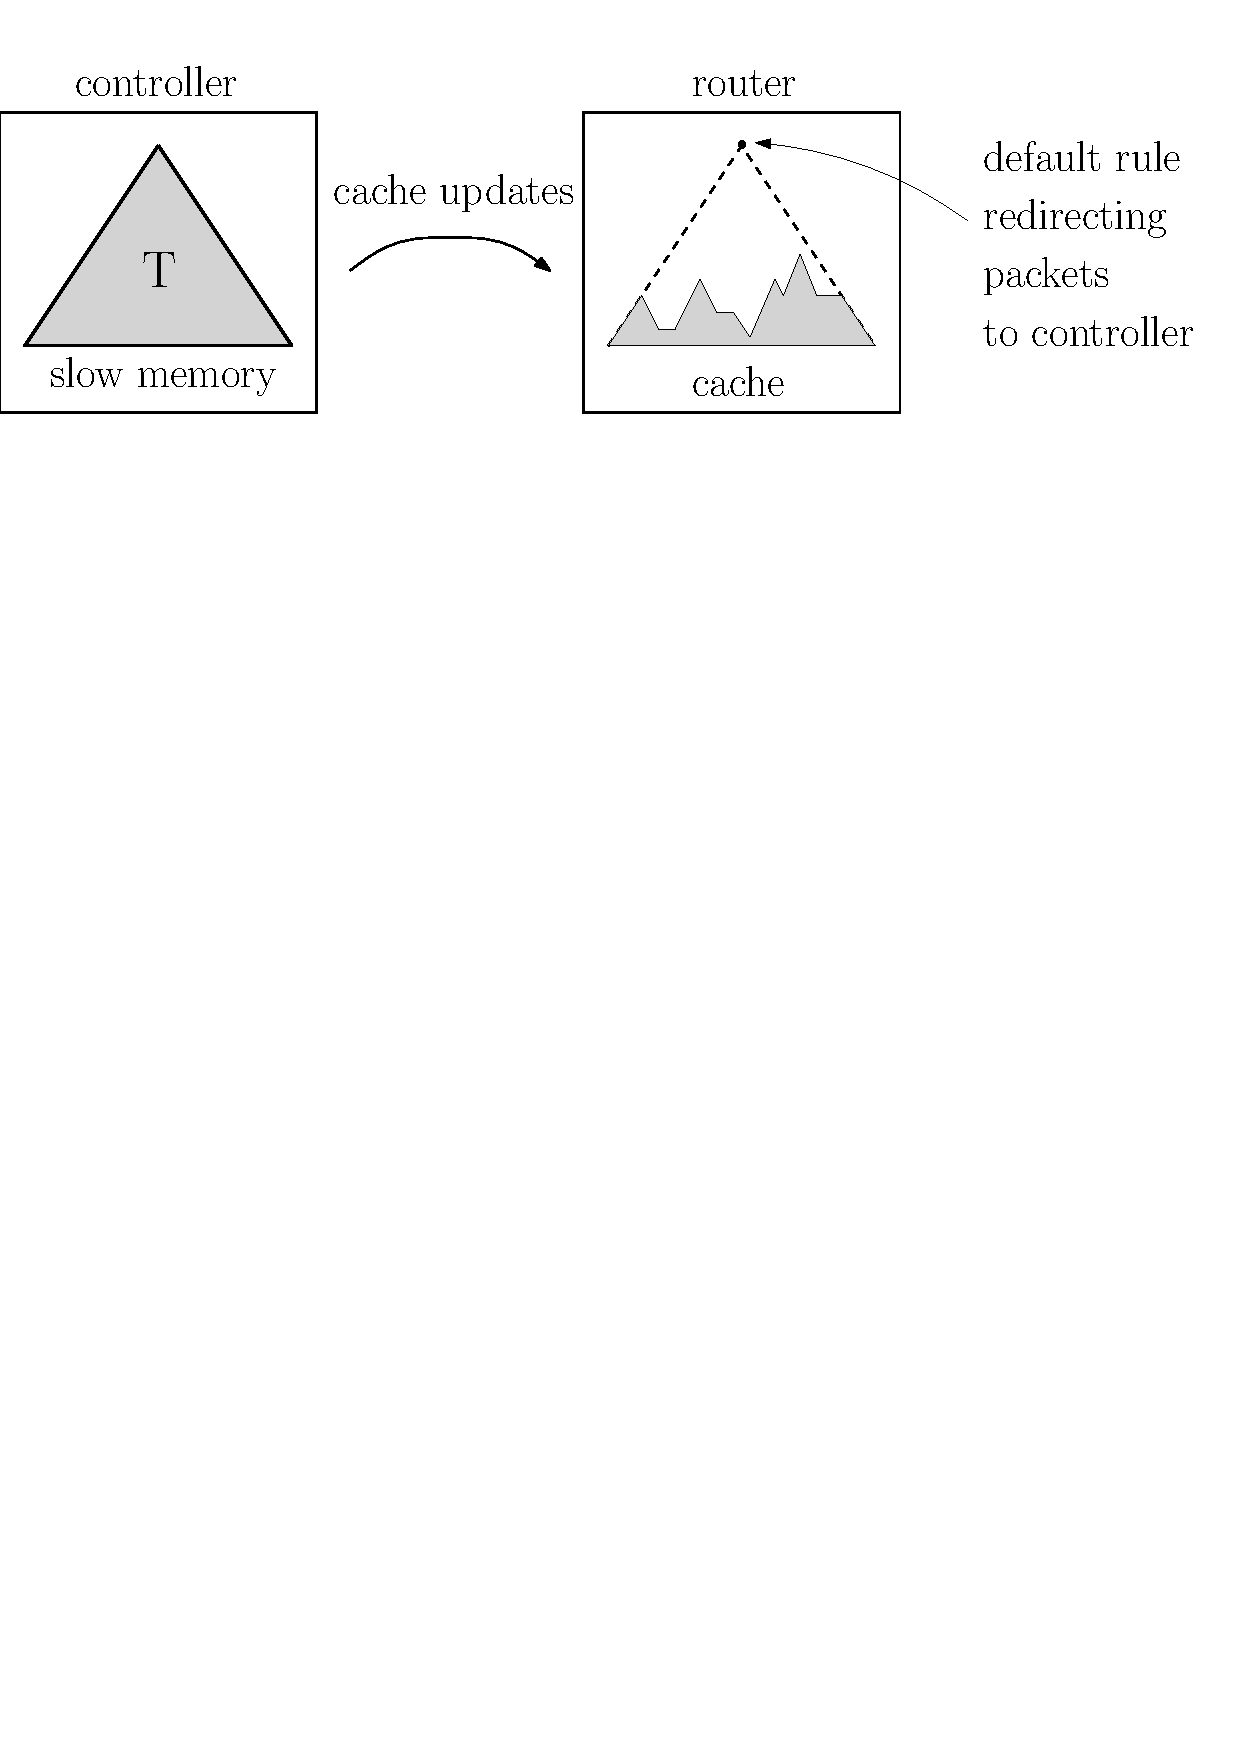
\includegraphics[width=0.9\columnwidth,keepaspectratio]{figs/cache-management/router}
  \caption{The router (\emph{right}) caches only a subset of all rules, and
  rules that are not cached are answered by the controller (\emph{left}) that
  keeps the whole tree of rules. Updates to the rules are passed by the
  controller to the router.}
  \label{fig:motivation}
\end{figure}


\paragraph{Tree dependencies.}

Note that the technical feasibility of this solution heavily depends on the
rule dependencies. In the most ubiquitous scenario, the rules are prefixes of
IP addresses (they are bit strings). Whenever a packet arrives, the router
follows a longest matching prefix (LMP) scheme: it searches for the rule that
is a~prefix of the destination IP of the packet and among matching rules it
chooses the longest one. In other words, if the prefixes corresponding to
rules are stored in the tree\footnote{We do not have to assume that they are
actually stored in a real tree; this tree is implicit in the LMP scheme.},
then the tree is traversed from the root downwards, and the last found rule is
used. This explains why we require the cached nodes to form a subforest:
leaving a less specific rule on the router while evicting a more specific one
(i.e., keeping a~tree node in cache while evicting its descendant) will result
in a~situation where packets will be forwarded according to the less specific
rule, and hence potentially exit through the wrong port. The LMP scheme also
ensures that the described approach is implementable: one could simply add
an~artificial rule at the tree root in the router (matching an empty prefix).
This ensures that when no actual matching rule is found in the router (in the
cache), the packet will be forwarded according to this artificial rule to the
controller that stores all the rules and can handle all packets appropriately.

So far, the papers on IP rule caching avoided dependencies either assuming
that rules do not overlap (a~tree has a single level)~\cite{route-caching-flat} 
or by preprocessing the tree, so that the rules become
non-overlapping~\cite{prefix-caching,fib-caching-non-overlapping}.
Unfortunately, this could lead to a large inflation of the routing table. A
notable exception is a recent solution called CacheFlow~\cite{cacheflow}. The
CacheFlow model supports dependencies even in the form of directed acyclic
graphs. However, CacheFlow was evaluated only experimentally, and no
worst-case guarantees were given on the overall cost of caching. Our work
provides theoretical foundations for respecting tree dependencies.

\paragraph{Negative requests.}

Additionally, a rule may need to be updated. For example, due to a~change
communicated by a dynamic routing protocol (e.g., BGP) the action defined by
a~rule has to be modified. In either case, we have to update the rules at the
controller: we assume that this cost is zero. (This cost is unavoidable for
any algorithm, so such an assumption makes our problem only more difficult.)
Furthermore, if the rule is also stored at the router, then we have to pay a~fixed
cost of $\alpha$ for updating the router (see the remark for the cost of
fetches and evictions). Such penalties can be easily simulated in our model:
we issue a~sequence of $\alpha$ negative requests to the updated node.  It is
straightforward to show that the costs in these two models can differ by a
factor of at most $2$. For a~formal argument, see
\lref[Appendix]{sec:bisimulation}.

\paragraph{Implementability.}

Note that the whole input (fed to a tree caching algorithm) is created at the
controller: positive requests are caused by cache misses (which redirect
packet to the controller) and batches of $\alpha$ negative requests are caused
by updates sent to the dynamic routing algorithm run at the controller.
Therefore, the whole tree caching algorithm can be implemented in software
in the controller only. Furthermore, our algorithm is a simple counter-based
scheme, which can be implemented efficiently and also fine-tuned for speed,
see \lref[Section]{sec:implementing_counters}.

\paragraph{Other work on forwarding table minimization.}

Other approaches for minimizing the number of stored rules were mostly based
on \emph{rules compression (aggregation)}, where the set of rules was replaced
by another equivalent and smaller set. Optimal aggregation of a fixed routing
table can be achieved by dynamic
programming~\cite{ortc,fib-compression-two-dimensional}, but the main
challenge lies in balancing the achieved compression and the amount of changes
to the routing table in the presence of \emph{updates} to this table. While
many practical heuristics have been devised by the networking community for
this problem~\cite{mms,fib-compression-fifa,fib-compression-globecom10,fib-compression-infocom13,fib-sigcomm,fib-compression-smalta,fib-compression-infocom10},
worst-case analyses were presented only for some restricted
scenarios~\cite{fib-icdcs,fib-sirocco}. Combining rules compression and rules
caching is so far an unexplored area.



\subsection{Virtual Clusters and Organization of Datacenters}


\begin{enumerate}
  \item Physical datacenter architecture and physical clusters
  \item Sharing datacenter resources and isolation requirements
\end{enumerate}

\url{https://technet.microsoft.com/en-us/library/hh965746.aspx}


Virtualized datacenters offer great flexibilities in terms of resource allocation. In particular, by
decoupling applications from the constraints of the underlying infrastructure, virtualization
supports an optimized mapping of virtual machines as well as their interconnecting network
 (the so-called \emph{virtual cluster})
to their
physical counterparts: a graph embedding problem.

However, existing virtual cluster embedding algorithms often ignore a crucial dimension of the problem, namely \emph{data locality}:
the input to a cloud application such as MapReduce is typically stored in a distributed,
and sometimes redundant, file system. Since moving
data is costly, an embedding algorithm should be data locality aware,
and allocate computational resources close to the data; in case of redundant storage, the algorithm should also optimize the \emph{replica selection}.

This paper initiates the algorithmic study of data locality aware virtual cluster embeddings
on datacenter topologies.
We
show that
despite the multiple degrees of freedom in terms of embedding, replica selection and assignment,
many problems can be
solved efficiently. We also highlight the limitations of such optimizations,
by presenting several NP-hardness proofs; interestingly,
our hardness results also hold in uncapacitated networks of small diameter.

\subsubsection{VC practical motivations}

Our model is motivated by batch-processing applications such as MapReduce.
Such applications use multiple virtual machines to
process data, often redundantly stored in a distributed file system implemented
by multiple servers~\cite{local-schedule-1,mapreduce}.
Datacenter networks are typically organized as fat-trees, with servers are
located at the tree leaves and inner nodes being switches or routers.
Given the amount of multiplexing over the mesh of links
and the availability of multi-path routing protocol, e.g.~ECMP, the redundant
links can be considered as a single aggregate link for bandwidth
reservations~\cite{oktopus,infocom16,ccr15emb,proteus}.

During execution, batch-processing applications typically cycle through different phases,
most prominently, a map phase and a reduce phase; between the two phases,
a shuffling operation is performed, a phase where the results from the mappers
are communicated to the reducers. Since the shuffling phase can constitute a
non-negligible part of the overall runtime~\cite{orchestra},
and since concurrent network transmissions can introduce interference and
performance unpredictability~\cite{amazonbw}, it is important
to provide explicit minimal bandwidth guarantees~\cite{talk-about}.
In particular, we model the virtual network connecting the virtual machines
as a virtual cluster~\cite{oktopus,talk-about,proteus};
however, we extend this model with a notion of data-locality.
In particular, we distinguish between the bandwidth needed between the assigned chunk
and virtual machine ($\CostTrans$) and the bandwidth needed between
two virtual machines ($\CostCom$). 


\subsubsection{OBR abstract}

This paper initiates the study of the classic balanced graph partitioning
problem from an online perspective: Given an~arbitrary sequence of pairwise
communication requests between~$n$ nodes, with patterns that may change over
time, the objective is~to~service these requests efficiently by partitioning
the nodes into~$\ell$ clusters, each of size~$k$, such that frequently
communicating nodes are located in the same cluster. The partitioning can be
updated dynamically by \emph{migrating} nodes between clusters. The goal is to
devise online algorithms which jointly minimize the amount of inter-cluster
communication and migration cost.

The problem features interesting connections to other well-known online
problems. For example, scenarios with~$\ell=2$ generalize online paging, and
scenarios with~$k=2$ constitute a~novel online variant of maximum matching. We
present several lower bounds and algorithms for settings both with and without
cluster-size augmentation. In particular, we prove that any deterministic
online algorithm has a competitive ratio of at least~$k$, even with
\emph{significant} augmentation. Our main algorithmic contributions are
an~$O(k \log{k})$-competitive deterministic algorithm for the general setting
with constant augmentation, and a constant competitive algorithm for the
maximum matching variant.


\subsubsection{OBR practical motivations}


There are many applications to the dynamic graph clustering problem.
To give just one example, we consider server virtualization in
datacenters. Distributed cloud applications, including batch processing
applications such as MapReduce, streaming applications such as Apache Flink or
Apache Spark, and scale-out databases and key-value stores such as Cassandra,
generate a significant amount of network traffic and a considerable fraction
of their runtime is due to network acti\-vi\-ty~\cite{MogPop12}. For example,
traces of jobs from a Facebook cluster reveal that network transfers on
average account for 33\% of the execution time~\cite{ChZMJS11}. In such
applications, it is desirable that frequently communicating virtual machines
are \emph{collocated}, i.e., mapped to the same physical server, since
communication across the network (i.e., inter-server communication) induces
network load and latency. However, migrating virtual machines between servers
also comes at a price: the state transfer is bandwidth intensive, and may even
lead to short service interruptions. Therefore the goal is to design online
algorithms that find a good trade-off between the inter-server communication
cost and the migration cost.






\section{Methods of Measuring the Quality of Results}

\subsection{Online Algorithms and Competitive Analysis}

Sleator, Tarjan: list update \cite{competitive-analysis}
Borodin book \cite{borodin-book}

\subsection{Time and Space Complexity and NP-completeness}
